\section{Redes Neurais}
\subsection{O que são Redes Neurais?}
\label{subsec:oquesaoredesneurais}

As redes neurais artificiais, como conhecidas na literatura \cite{haykin2004comprehensive, haykin2009neural, lecun2015deep}, são estruturas aptas ao aprendizado inspiradas na forma com que os neurônios de cérebros reais funcionam. Um modo estrutural de organização, bem como a distribuição de informação ao longo da arquitetura foram levados em conta na construção deste poderoso modelo matemático que hoje conhecemos como Redes Neurais \cite{haykin2004comprehensive, haykin2009neural, lecun2015deep}. Tais redes são reconhecidamente uma tecnologia bioinspirada, já que são profundamente motivadas pelo aprendizado demonstrado pelo cérebro de seres vivos, notadamente o dos seres humanos. 
\begin{figure}[b]
    \centering
    \includegraphics[scale=0.17]{Figuras/Cap2/neuronio.png}
        \caption{Representação de um neurônio. Figura \ref{fig:neuronio} extraída do site \cite{Pixabay} e editada pelo autor. O site \cite{Pixabay} é uma plataforma gratuita de distribuição de imagens, ou seja, o uso das imagens não ferem direitos autorais.}
        \label{fig:neuronio}
\end{figure}


A Figura \ref{fig:neuronio} representa um neurônio utilizado como componente fundamental das redes neurais artificiais. Para entender como essa representação nos leva ao modelo matemático, devemos primeiro descrever suas quatro partes principais, bem como a função de cada parte do neurônio.

\begin{enumerate}
    \item núcleo: onde é processada a informação;
    \item dendrito: de onde vem a informação a ser processada (ou seja, o \textit{input});
    \item axônio: parte que o neurônio usa para enviar sinais (ou seja, o \textit{output});
    \item terminal do axônio: onde a informação de saída é propagada para os demais neurônios da rede ou utilizada como resposta final da rede.
\end{enumerate}

Uma rede neural artificial é implementada por meio da conexão de diversos neurônios, cujos axônios se conectam ao dendritos de outro, levando o sinal processado pelo núcleo. Os neurônios recebem tal sinal em seus dendritos os quais, por sua vez, processam o sinal em seus núcleos, enviando novamente o resultado (via axônios) para os próximos neurônios, por meio dos terminais dos axônios. Eis a lógica de propagação e processamento de informação que as redes neurais artificiais almejam emular.

Este trabalho tem como motivação o uso de Redes Neurais pelos benefícios que elas trazem para o problema específico da previsão de valores do Bitcoin. A motivação biológica não faz parte das motivações deste trabalho.

A próxima subseção apresentará a representação gráfica e matemática de uma Rede Neural, que será usada no decorrer deste trabalho.

\subsection{Representação de uma Rede Neural}

\subsubsection{Representação de um Neurônio}
\label{subsubsec:representacaoumneuronio}

No objetivo de representar mais formalmente o processamento matemático empreendido por uma Rede Neural, vamos transformar as quatro principais partes do neurônio da subseção \ref{subsec:oquesaoredesneurais} em um diagrama. A Figura \ref{fg:rede_neural_simples} apresenta o diagrama de um neurônio, no qual podemos elencar os componentes seguintes:
\begin{enumerate}
 \item dendrito (\textit{input}): representado pelos círculos azuis. Cada círculo contém o valor referente à sua amostra $x_n$; nesse exemplo, $n = 3$ amostras. A informação de cada uma das $n$ amostras é enviada para o núcleo;
    \item núcleo: representado pelo círculo laranja. No núcleo, as amostras $x_n$ e os pesos $\theta_n$ executam a chamada \textbf{função de ativação}, apresentada na Seção \ref{sec:funcaoativacao};
   
    \item axônio (\textit{output}): consiste na saída do núcleo, a qual armazena o resultado da operação;
    \item terminal do axônio: descreve a transformação da saída num (\textit{input}) de um novo neurônio, geralmente da camada posterior.
    
\end{enumerate}


\begin{figure}
\centering
\large
\begin{tikzpicture}[shorten >=1pt,->,draw=black!70, node distance=\layersep]
    \tikzstyle{every pin edge}=[<-,shorten <=1pt]
    \tikzstyle{neuron}=[circle,fill=black!50,minimum size=05pt,inner sep=15pt]
    \tikzstyle{input neuron}=[neuron, fill=blue!50];
    \tikzstyle{output neuron}=[neuron, fill=orange!50, inner sep=10pt];

    \tikzstyle{annot} = [text width=4em, text centered]

    % Draw the input layer nodes
    \foreach \name / \y in {1,...,3}
    % This is the same as writing \foreach \name / \y in {1/1,2/2,3/3,4/4}
        \node[input neuron, pin=left:] (I-\name) at (0,-2.2*\y){x\y};

    % Draw the output layer node
    \node[output neuron,pin={[pin edge={->}]right:}, right of=I-1] (O) at (0,-4.4) { $h_\theta (x)$};

    % Connect every node in the hidden layer with the output layer
    \foreach \source in {1,...,3}
        \path (I-\source) edge (O);

    % Annotate the layers
   \node[annot,above of=I-1, node distance=1.7cm] (hl) {Entrada};
    \node[annot,right of=hl] {Saída};
    
    
\end{tikzpicture}
\caption{Representação de um neurônio}
\label{fg:rede_neural_simples}
\end{figure}

Os elementos desse neurônio podem ser escritos na forma matricial. Assumindo uma entrada $x$ composta de $n$ elementos, podemos representá-la como:
\begin{equation}
  \mathbf{x}^T \triangleq \begin{bmatrix}x_{1}&x_{2}&x_{3}&...&x_{n-1}&x_{n} \end{bmatrix}
\end{equation}
 com os pesos representados como:
 \begin{equation}
  \mathbf{\theta}^T \triangleq \begin{bmatrix}\theta_{1}&\theta_{2}&\theta_{3}&...&\theta_{n-1}&\theta_{n}\end{bmatrix}
\end{equation}

Frequentemente na literatura \cite{haykin2004comprehensive, haykin2009neural, lecun2015deep} é adicionado em cada neurônio uma amostra extra, chamada de \textit{bias}, ou viés. O \textit{bias} serve para aumentar os graus de liberdade do sistema, levando o resultado do Neurônio para uma determinada direção. Ele permite que restrições muito severas não sejam aplicadas ao sistema. Por exemplo, caso as entradas sejam nulas, o neurônio terá uma saída também nula, o que comumente é uma restrição muito forte. O  \textit{bias}, portanto,  permite uma melhor adaptação do sistema.

%FEITO
%\dbh{Errado, Bernardo! Esse bias é essencial, porque caso contrário a rede neural necessariamente irá jogar uma entrada nula numa saída também nula, o que comumente é uma restrição muito forte!!!}

\subsubsection{Representação de uma Rede Neural}
\label{subsubsec:representacaoumaredeneural}
Nas seção \ref{subsubsec:representacaoumneuronio} foi apresentado a representação de um Neurônio. Nesta seção, será empregada a representação da seção anterior para definir uma Rede Neural, que será usada como modelo no restante deste trabalho. A expansão da representação de \ref{subsubsec:representacaoumneuronio} permite uma descrição global de uma rede neural artificial. A Figura \ref{fg:rede_neural_generica} representa uma Rede Neural. Essa rede possui $n$ componentes de entrada, $m$ neurônios em cada uma das $k$ camadas, onde $n, m, k\in \mathbb{N}$. Cada neurônio aplica uma função não linear nas entradas que recebe; normalmente tal função pode ser a sigmoidal (\ref{subsec:sigmoid}), a tangente hiperbólica (\ref{subsec:htan}) ou a ReLu (\ref{subsec:relu}), que serão abordadas especificamente na seção \ref{sec:funcaoativacao}.

%--

\begin{figure}
\centering
\large
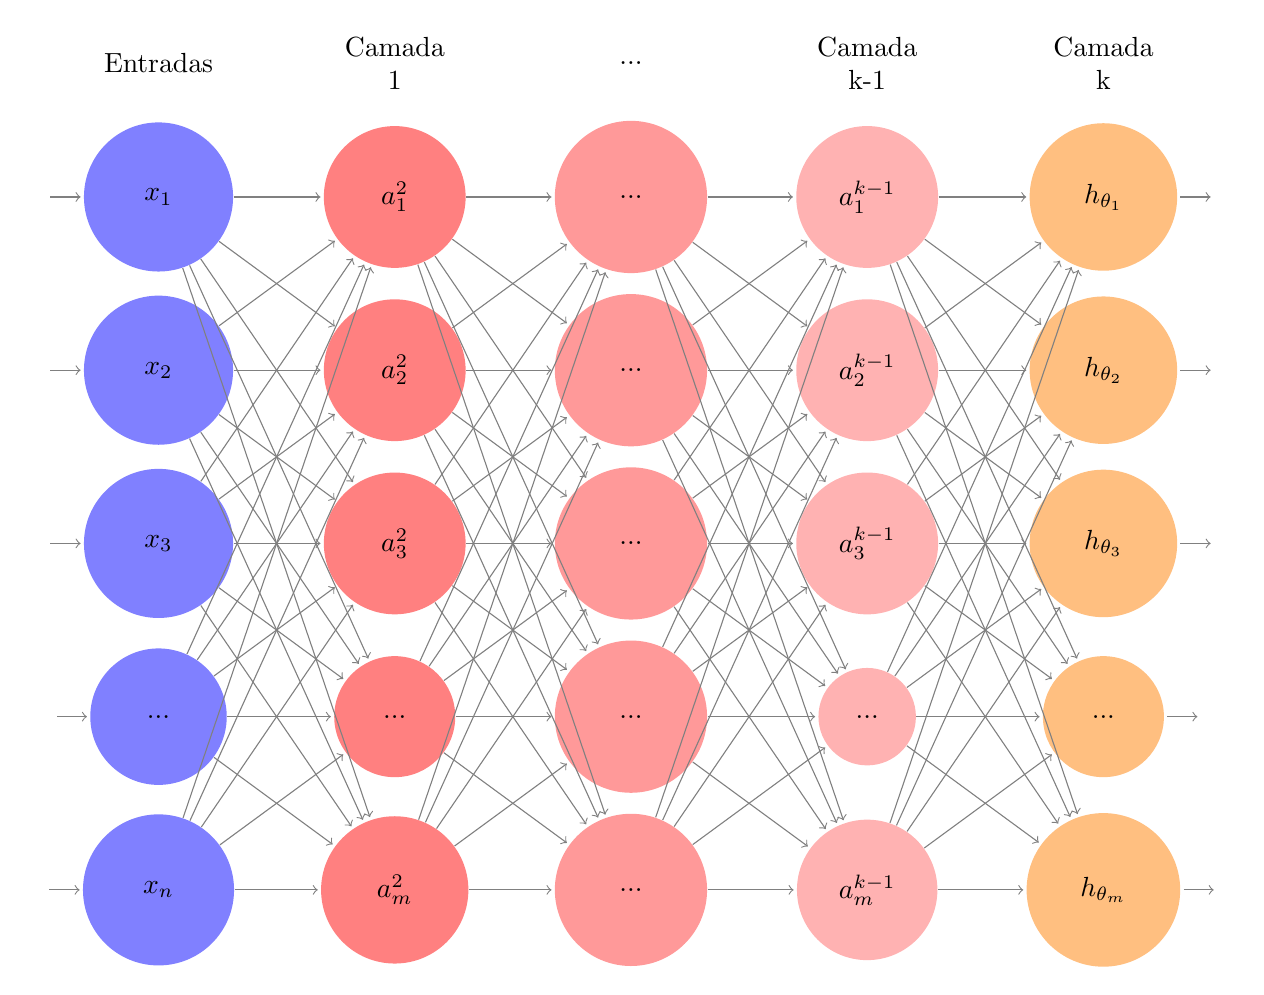
\begin{tikzpicture}[shorten >=1pt,->,draw=black!50, node distance=\layersep]
    \tikzstyle{every pin edge}=[<-,shorten <=1pt]
    \tikzstyle{neuron}=[circle,fill=black!25,minimum size=17pt,inner sep=15pt]
    \tikzstyle{input neuron}=[neuron, fill=blue!50];
    \tikzstyle{output neuron}=[neuron, fill=orange!50,inner sep=13pt];
    \tikzstyle{hidden neuron}=[neuron, fill=red!50,inner sep=13pt];
     \tikzstyle{hidden_n neuron}=[neuron, fill=red!30,inner sep=10pt];
     \tikzstyle{p neuron}=[neuron, fill=red!40,inner sep=17pt];
    \tikzstyle{annot} = [text width=4em, text centered]
    
    \node[input neuron, pin=left:] (I-1) at (-5,-2.2*1) {$x_1$};
    \node[input neuron, pin=left:] (I-2) at (-5,-2.2*2) {$x_2$};
    \node[input neuron, pin=left:] (I-3) at (-5,-2.2*3) {$x_3$};
    \node[input neuron, pin=left:] (I-4) at (-5,-2.2*4) {...};
    \node[input neuron, pin=left:] (I-5) at (-5,-2.2*5) {$x_n$};
    
    \node[hidden neuron] (H-1) at (-2,-2.2*1) {$a_1^2$};
    \node[hidden neuron] (H-2) at (-2,-2.2*2) {$a_2^2$};
    \node[hidden neuron] (H-3) at (-2,-2.2*3) {$a_3^2$};
    \node[hidden neuron] (H-4) at (-2,-2.2*4) { ... };
    \node[hidden neuron] (H-5) at (-2,-2.2*5) {$a_m^2$};
    
    \node[p neuron] (p-1) at (1,-2.2*1) { ... };
    \node[p neuron] (p-2) at (1,-2.2*2) { ... };
    \node[p neuron] (p-3) at (1,-2.2*3) { ... };
    \node[p neuron] (p-4) at (1,-2.2*4) { ... };
    \node[p neuron] (p-5) at (1,-2.2*5) { ... };

    \node[hidden_n neuron] (Hn-1) at (4,-2.2*1) {$a_1^{k-1}$};
    \node[hidden_n neuron] (Hn-2) at (4,-2.2*2) {$a_2^{k-1}$};
    \node[hidden_n neuron] (Hn-3) at (4,-2.2*3) {$a_3^{k-1}$};
    \node[hidden_n neuron] (Hn-4) at (4,-2.2*4) { ... };
    \node[hidden_n neuron] (Hn-5) at (4,-2.2*5) {$a_{m}^{k-1}$};
    
    \node[output neuron,pin={[pin edge={->}]right:}] (O-1) at (7,-2.2*1) { $h_{\theta_1}$};
    \node[output neuron,pin={[pin edge={->}]right:}] (O-2) at (7,-2.2*2) { $h_{\theta_2}$};
    \node[output neuron,pin={[pin edge={->}]right:}] (O-3) at (7,-2.2*3) { $h_{\theta_3}$};
    \node[output neuron,pin={[pin edge={->}]right:}] (O-4) at (7,-2.2*4) { ... };
    \node[output neuron,pin={[pin edge={->}]right:}] (O-5) at (7,-2.2*5) { $h_{\theta_m}$};
    
    \foreach \source in {1,...,5}
        \foreach \dest in {1,...,5}
            \path (I-\source) edge (H-\dest);

    \foreach \source in {1,...,5}
        \foreach \dest in {1,...,5}
            \path (H-\source) edge (p-\dest);
            
    \foreach \source in {1,...,5}
        \foreach \dest in {1,...,5}
            \path (p-\source) edge (Hn-\dest);
    
    \foreach \source in {1,...,5}
        \foreach \dest in {1,...,5}
            \path (Hn-\source) edge (O-\dest);

    \node[annot] at (-5,-0.5) {Entradas};
    \node[annot] at (-2,-0.5){Camada 1};
    \node[annot] at (1, -0.5){...};
    \node[annot] at (4, -0.5){Camada k-1};
    \node[annot] at (7, -0.5){Camada k};
\end{tikzpicture}
\caption{Representação de uma Rede Neural}
\label{fg:rede_neural_generica}
\end{figure}


Para representar a Rede Neural, primeiramente, é preciso  representar $a^{(x)}_y$, que é chamada de \textbf{ativação}. A ativação é individual para cada Neurônio, onde $a^{(x)}_y$ é a ativação referente ao Neurônio da camada $x$, ficando a cargo de $y$ identificar o Neurônio dentro de todos os possíveis Neurônios da camada $x$. A \textbf{ativação} é calculado realizando a soma de todas as entradas de determinado Neurônio, multiplicadas pelos seus respectivos pesos, que servem de entrada para a função de ativação, que é o resultado do Neurônio em questão. Feito esse processo, podemos representar $a^{(x)}_y$ usando a equação \ref{fun:axy}.
\begin{equation}
    a^{(x)}_y=g(\Theta^{(x-1)}_{y0}x{}_0+\Theta^{(x-1)}_{y1}x{}_1+\Theta^{(x-1)}_{y2}x{}_2\Theta^{(x-1)}_{y3}x{}_3+...+\Theta^{(x-1)}_{y(m-1)}x{}_{m-1}+\Theta^{(x-1)}_{ym}x{}_m )
    \label{fun:axy}
\end{equation}


Sabendo como calcular os $a^{(x)}_y$ de todas as camadas, deixando claro que é preciso saber o resultado da camada anteriora para calcular a camada atual, é possível definir uma saída genérica $\mathbf{h}{\Theta}(x)_y$ como na  Eq. \ref{fun:thetanm}. Note que a Eq. \ref{fun:thetanm} é apenas consequência de ir executando a Eq.  \label{fun:axy} até a última camada. Esse procedimento é conhecido como \textit{Forward Propagagtion}, e será abordado melhor na seção \ref{subsec:backpropagation} ao falar de Backpropagation.

\begin{equation}
    \mathbf{h}{\Theta}(x) = a^{(n)}_y = g(\Theta^{n-1}_{y0}a^{n-1}_{0}+\Theta^{n-1}_{y1}a^{n-1}_{1}+\Theta^{n-1}_{y2}a^{n-1}_{2}+...+\Theta^{n-1}_{y(n-1)}a^{n-1}_{n-1}+\Theta^{n-1}_{yn}a^{n-1}_{m})
     \label{fun:thetanm}
\end{equation}


Para simplificar os cálculos, é usual utilizar operações matriciais, que conseguem atualizar todos os seus componentes em uma única operação. Para representar todas as entradas, por exemplo, foi utilizado a Eq. \ref{fun:entrada_generica}.
%FEITO
%\dbh{O texto está muito seco; só definições matemáticas, as quais não apelam à intuição!}


\begin{equation}
    \label{fun:entrada_generica}
  \mathbf{x}^T = \begin{bmatrix}x_{1}&x_{2}&x_{3}&...&x_{n-1}&x_{n}\end{bmatrix}
\end{equation}

E a resposta da Rede Neural Genérica pode ser escrita na forma matricial mediante o emprego de \eqref{fun:h_generica}.

 \begin{equation}
   \label{fun:h_generica}
   \mathbf{h}\theta(x) = 
   \begin{bmatrix}
   g(\Theta^{(n-1)}_{10}a^{(n-1)}_{0}+\Theta^{(n-1)}_{11}a^{(n-1)}_{1}+ ... +\Theta^{(n-1)}_{1(m-1)}a^{(n-1)}_{(m-1)} )\\
   g(\Theta^{(n-1)}_{20}a^{(n-1)}_{0}+\Theta^{(n-1)}_{21}a^{(n-1)}_{1}+ ... +\Theta^{(n-1)}_{2(m-1)}a^{(n-1)}_{(m-1)} )\\
   g(\Theta^{(n-1)}_{30}a^{(n-1)}_{0}+\Theta^{(n-1)}_{31}a^{(n-1)}_{1}+ ... +\Theta^{(n-1)}_{3(m-1)}a^{(n-1)}_{(m-1)} )\\
    \vdots\\
    g(\Theta^{(n-1)}_{(m-1)0}a^{(n-1)}_{0}+\Theta^{(n-1)}_{(m-1)1}a^{(n-1)}_{1}+ ... +\Theta^{(n-1)}_{(m-1)}a^{(n-1)}_{(m-1)} )\\
    
   \end{bmatrix} 
\end{equation}


Essas são as representações gráficas e matemáticas que serão utilizadas no decorrer deste trabalho. Na próxima subseção será abordada a função de ativação.

\subsection{Funções de Ativação}
\label{sec:funcaoativacao}

\cite{activationfun}

\dbh{Motivar o emprego da função não-linear; a não linearidade é muito importante para o poder das redes neurais.}

\bac{motivar mais as funcoes de ativacao **ReLU copiada do guilherme}

A função de ativação é denotada como $h_\Theta (x)$ e define a saída de um neurônio para uma dada entrada $x$. Descreveremos a seguir a função de ativação sigmoide, a mais comum em Redes Neurais \cite{haykin2004comprehensive, haykin2009neural, lecun2015deep}.

\subsubsection{Função Sigmoide}
\label{subsec:sigmoid}
\dbh{Não, mil vezes não! A sigmoide é suave, não é brusca como mostrado na equação (23)! Este capítulo tem que ser muito lapidado. Só tem definições matemáticas, com pouca discussão motivadora! Ler mais!}

A Eq.\eqref{fun:sigmoid} representa a função sigmoide, apresentada graficamente na Fig. \ref{fg:funcao_sigmoide}. 


\begin{equation}
  f(x) =  \frac{\mathrm{1} }{\mathrm{1} + e^{- \mathbf{\theta^T}x}}
  \label{fun:sigmoid}
\end{equation}

\begin{center}
    \begin{figure}
        \centering
        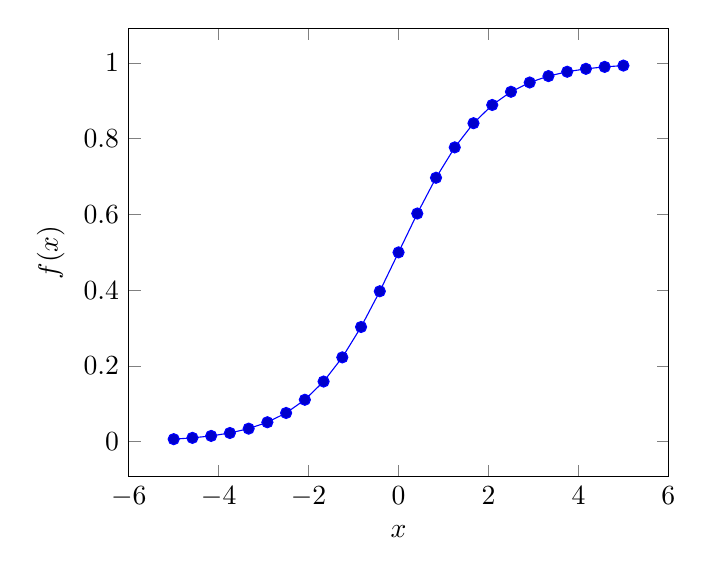
\begin{tikzpicture}
        	\begin{axis}[
        		xlabel=$x$,
        		ylabel={$f(x)$}
        	]
        	\addplot {1 / (1 + e^-x)};
        	\end{axis}
        \end{tikzpicture}
    \caption{Função Sigmoide}\label{fg:funcao_sigmoide}
	\end{figure}
\end{center}

\subsubsection{Função Tangente Hiperbólica}
\label{subsec:htan}
\bac{TANGENTE HIPERBOLCIA}

\begin{equation}
  f(x) =  \frac{\mathrm{1} - e^{- \mathbf{\theta^T}x}}{\mathrm{1} + e^{- \mathbf{\theta^T}x}}
  \label{fun:sigmoid}
\end{equation}

\begin{center}
    \begin{figure}
        \centering
        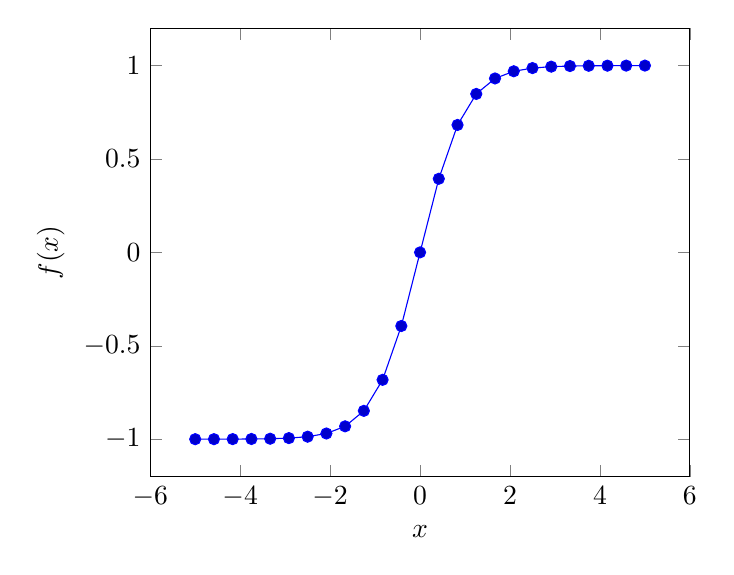
\begin{tikzpicture}
        	\begin{axis}[
        		xlabel=$x$,
        		ylabel={$f(x)$}
        	]
        	\addplot {(e^x - e^-x) / (e^x + e^-x)};
        	\end{axis}
        \end{tikzpicture}
    \caption{Função Tangente Hiperbólica}\label{fg:funcao_tanh}
	\end{figure}
\end{center}



\subsubsection{Função ReLU}
\label{subsec:relu}
A função ReLU (\textit{rectified linear unit}) realiza a ativação do nó apenas se a entrada estiver acima de um valor predeterminado. O ReLU é representado pela equação $\phi (x) = max(0,x)$. A Figura \ref{fig:relu} mostra o gráfico dessa função. Trata-se de uma função não linear (ainda que linear por partes) que permite implementações com baixo custo computacional.

\begin{figure}[!htb]
    \centering
    
    \begin{tikzpicture}
    \begin{axis}[
        		xlabel=$x$,
        		ylabel={$f(x)$}
        	]
        \addplot+[mark=none,blue,domain=-3:0] {0};
        \addplot+[mark=none,blue,domain=0:4] {x};
    \end{axis}
\end{tikzpicture}
\caption{Função ReLU. \label{fig:relu}}
\end{figure}